\documentclass[border=5pt]{standalone}
\usepackage{fontspec}
\usepackage{unicode-math}
\setmainfont{Noto Serif}
\newfontfamily\FigureItalic{Noto Serif}
\setmathfont{STIXTwoMath-Regular.otf}
\usepackage{tikz}
\usetikzlibrary{arrows.meta,calc,patterns,decorations.pathmorphing,decorations.markings,decorations.pathreplacing,positioning,backgrounds}
\definecolor{Ink}{HTML}{000000}
\definecolor{Curve}{HTML}{000000}
\definecolor{Bzero}{HTML}{000000}
\definecolor{Bone}{HTML}{000000}
\definecolor{Btwo}{HTML}{000000}
\definecolor{Bthree}{HTML}{000000}
\definecolor{Bfour}{HTML}{000000}
\tikzset{
 ax/.style={draw=Ink,line width=.72pt,-{Latex[length=2.4mm,width=1.5mm]}},
 lev/.style={draw=Ink,line width=1.4pt,line cap=butt},
 thinlev/.style={draw=Ink,line width=.65pt,line cap=butt},
 helper/.style={draw=Ink,line width=.65pt},
 bare/.style={draw=Ink,line width=.95pt,dash pattern=on 4pt off 2.8pt},
 curve/.style={draw=Ink,line width=1.85pt,line cap=round,line join=round},
 ray/.style={draw=Ink,line width=1.0pt,-{Latex[length=2.3mm,width=1.4mm]}},
 measure/.style={draw=Ink,line width=.75pt,{Latex[length=1.9mm,width=1.2mm]}-{Latex[length=1.9mm,width=1.2mm]}},
 link/.style={draw=Ink,line width=1.0pt},
 wave/.style={draw=Ink,line width=.85pt,decorate,decoration={snake,amplitude=.33mm,segment length=2.5mm,pre length=.8mm,post length=.8mm}},
 photon/.style={draw=Ink,line width=1.0pt,-{Latex[length=2.0mm,width=1.3mm]},decorate,decoration={snake,amplitude=.4mm,segment length=2.7mm,pre length=0mm,post length=1.9mm}},
 lab/.style={text=Ink,font=\fontsize{13.5}{16}\selectfont,inner sep=2pt},
 small/.style={text=Ink,font=\fontsize{11.5}{14}\selectfont,inner sep=2pt},
 tag/.style={text=Ink,font=\fontsize{14}{17}\selectfont\FigureItalic\itshape,inner sep=2pt}}
\pagestyle{empty}

\begin{document}
% Figure 13.10; source-grounded revision.
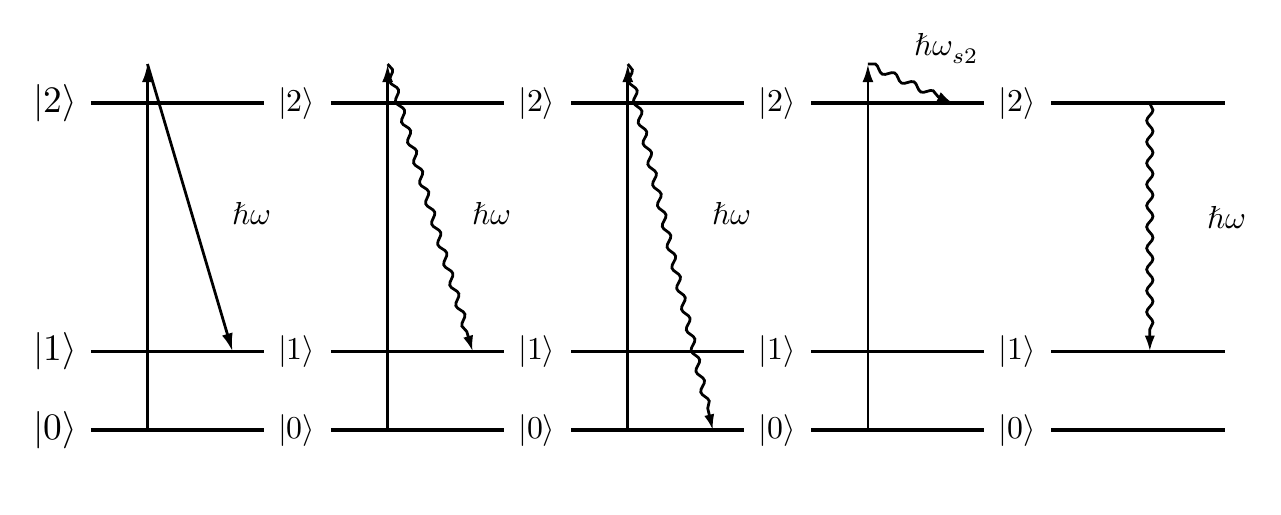
\begin{tikzpicture}[x=1cm,y=1cm]
\coordinate (e0_0) at (1.00000,0.00000);
\coordinate (e0_0L) at (-0.10000,0.00000);
\coordinate (e0_0R) at (2.10000,0.00000);
\draw[lev] (e0_0L) -- (e0_0R);
\node[lab,anchor=east] at (-0.20000,0.00000) {$|0\rangle$};
\coordinate (e0_1) at (1.00000,1.00000);
\coordinate (e0_1L) at (-0.10000,1.00000);
\coordinate (e0_1R) at (2.10000,1.00000);
\draw[lev] (e0_1L) -- (e0_1R);
\node[lab,anchor=east] at (-0.20000,1.00000) {$|1\rangle$};
\coordinate (e0_2) at (1.00000,4.15000);
\coordinate (e0_2L) at (-0.10000,4.15000);
\coordinate (e0_2R) at (2.10000,4.15000);
\draw[lev] (e0_2L) -- (e0_2R);
\node[lab,anchor=east] at (-0.20000,4.15000) {$|2\rangle$};
\coordinate (virtual0) at (0.62000,4.65000);
\draw[ray] (0.62000,0.00000) -- (virtual0);
\draw[ray] (virtual0) -- (1.70000,1.00000);
\node[small] at (1.95000,2.70000) {$\hbar\omega_{\mathrm{ст}}$};
\node[tag] at (1.00000,-0.65000) {а};
\coordinate (e1_0) at (4.05000,0.00000);
\coordinate (e1_0L) at (2.95000,0.00000);
\coordinate (e1_0R) at (5.15000,0.00000);
\draw[lev] (e1_0L) -- (e1_0R);
\coordinate (e1_1) at (4.05000,1.00000);
\coordinate (e1_1L) at (2.95000,1.00000);
\coordinate (e1_1R) at (5.15000,1.00000);
\draw[lev] (e1_1L) -- (e1_1R);
\coordinate (e1_2) at (4.05000,4.15000);
\coordinate (e1_2L) at (2.95000,4.15000);
\coordinate (e1_2R) at (5.15000,4.15000);
\draw[lev] (e1_2L) -- (e1_2R);
\coordinate (virtual1) at (3.67000,4.65000);
\draw[ray] (3.67000,0.00000) -- (virtual1);
\draw[photon] (virtual1) -- (4.75000,1.00000);
\node[small] at (5.00000,2.70000) {$\hbar\omega_{\mathrm{ст}}$};
\node[tag] at (4.05000,-0.65000) {б};
\coordinate (e2_0) at (7.10000,0.00000);
\coordinate (e2_0L) at (6.00000,0.00000);
\coordinate (e2_0R) at (8.20000,0.00000);
\draw[lev] (e2_0L) -- (e2_0R);
\coordinate (e2_1) at (7.10000,1.00000);
\coordinate (e2_1L) at (6.00000,1.00000);
\coordinate (e2_1R) at (8.20000,1.00000);
\draw[lev] (e2_1L) -- (e2_1R);
\coordinate (e2_2) at (7.10000,4.15000);
\coordinate (e2_2L) at (6.00000,4.15000);
\coordinate (e2_2R) at (8.20000,4.15000);
\draw[lev] (e2_2L) -- (e2_2R);
\coordinate (virtual2) at (6.72000,4.65000);
\draw[ray] (6.72000,0.00000) -- (virtual2);
\draw[photon] (virtual2) -- (7.80000,0.00000);
\node[small] at (8.05000,2.70000) {$\hbar\omega_{\mathrm{РР}}$};
\node[tag] at (7.10000,-0.65000) {в};
\coordinate (e3_0) at (10.15000,0.00000);
\coordinate (e3_0L) at (9.05000,0.00000);
\coordinate (e3_0R) at (11.25000,0.00000);
\draw[lev] (e3_0L) -- (e3_0R);
\coordinate (e3_1) at (10.15000,1.00000);
\coordinate (e3_1L) at (9.05000,1.00000);
\coordinate (e3_1R) at (11.25000,1.00000);
\draw[lev] (e3_1L) -- (e3_1R);
\coordinate (e3_2) at (10.15000,4.15000);
\coordinate (e3_2L) at (9.05000,4.15000);
\coordinate (e3_2R) at (11.25000,4.15000);
\draw[lev] (e3_2L) -- (e3_2R);
\coordinate (virtual3) at (9.77000,4.65000);
\draw[ray] (9.77000,0.00000) -- (virtual3);
\draw[photon] (virtual3) -- (10.85000,4.15000);
\node[small] at (10.77000,4.85000) {$\hbar\omega_{s2}$};
\node[tag] at (10.15000,-0.65000) {г};
\coordinate (e4_0) at (13.20000,0.00000);
\coordinate (e4_0L) at (12.10000,0.00000);
\coordinate (e4_0R) at (14.30000,0.00000);
\draw[lev] (e4_0L) -- (e4_0R);
\coordinate (e4_1) at (13.20000,1.00000);
\coordinate (e4_1L) at (12.10000,1.00000);
\coordinate (e4_1R) at (14.30000,1.00000);
\draw[lev] (e4_1L) -- (e4_1R);
\coordinate (e4_2) at (13.20000,4.15000);
\coordinate (e4_2L) at (12.10000,4.15000);
\coordinate (e4_2R) at (14.30000,4.15000);
\draw[lev] (e4_2L) -- (e4_2R);
\draw[photon] (13.35000,4.15000) -- (13.35000,1.00000);
\node[small,anchor=west] at (14.00000,2.65000) {$\hbar\omega_{\mathrm{ф}}$};
\node[tag] at (13.20000,-0.65000) {д};\node[small,anchor=east,fill=white,inner sep=.65pt] at (2.780,0.000) {$|0\rangle$};
\node[small,anchor=east,fill=white,inner sep=.65pt] at (2.780,1.000) {$|1\rangle$};
\node[small,anchor=east,fill=white,inner sep=.65pt] at (2.780,4.150) {$|2\rangle$};
\node[small,anchor=east,fill=white,inner sep=.65pt] at (5.830,0.000) {$|0\rangle$};
\node[small,anchor=east,fill=white,inner sep=.65pt] at (5.830,1.000) {$|1\rangle$};
\node[small,anchor=east,fill=white,inner sep=.65pt] at (5.830,4.150) {$|2\rangle$};
\node[small,anchor=east,fill=white,inner sep=.65pt] at (8.880,0.000) {$|0\rangle$};
\node[small,anchor=east,fill=white,inner sep=.65pt] at (8.880,1.000) {$|1\rangle$};
\node[small,anchor=east,fill=white,inner sep=.65pt] at (8.880,4.150) {$|2\rangle$};
\node[small,anchor=east,fill=white,inner sep=.65pt] at (11.930,0.000) {$|0\rangle$};
\node[small,anchor=east,fill=white,inner sep=.65pt] at (11.930,1.000) {$|1\rangle$};
\node[small,anchor=east,fill=white,inner sep=.65pt] at (11.930,4.150) {$|2\rangle$};
\end{tikzpicture}

\end{document}
